224. \begin{figure}[ht!]
\center{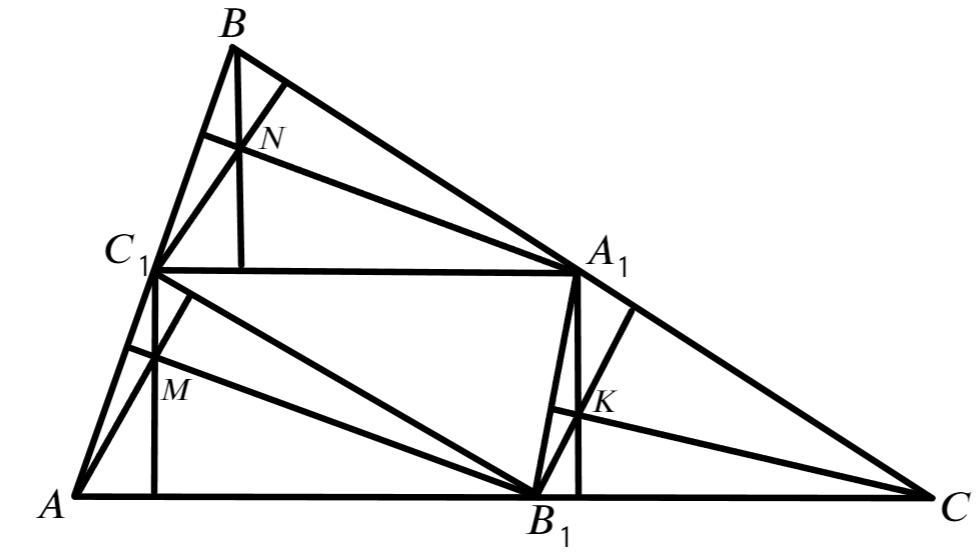
\includegraphics[scale=0.35]{g8-224.png}}
\end{figure}\\
Пусть $A_1,\ B_1,\ C_1$ --- середины сторон соответственно $BC,\ AC,\ AB$ остроугольного треугольника $ABC;$ пусть также перпендикуляры, опущенные из точки $C_1$ на $AC$ и из точки $B_1$ на $AB,$ пересекаются в точке $M;$ из точки $C_1$ на $BC$ и из точки $A_1$ на $AB$ --- в точке $N;$ из точки $A_1$ на $AC$ и из точки $B_1$ на $BC$ --- в точке $K.$ Тогда $M,\ N,\ K$ --- точки пересечения высот треугольников $AB_1C_1,\ BA_1C_1,\ CA_1B_1$ соответственно.

Треугольник $C_1MB_1$ равен треугольнику $BNA_1,$ а треугольник $A_1KB_1$ --- треугольнику $BNC_1$ (по стороне и двум прилежащим к ней углам). Следовательно,
$S_{A_1KB_1MC_1N} = S_{\Delta A_1B_1C_1} + S_{\Delta A_1NC_1} + S_{\Delta C_1MB_1} + S_{\Delta A_1KB_1}
= S_{\Delta A_1B_1C_1} + S_{\Delta A_1NC_1} + S_{\Delta BNA_1} + S_{\Delta BNC_1}
= S_{\Delta A_1B_1C_1} + S_{\Delta A_1BC_1} = \cfrac{1}{4}S_{\Delta ABC} + \cfrac{1}{4}S_{\Delta ABC} = \cfrac{1}{2}S_{\Delta ABC}=\cfrac{1}{2}\cdot 8=4.$\\
